\documentclass[journal]{IEEEtran}

\usepackage[T1]{fontenc}
\usepackage{amsmath}
\usepackage{amsfonts}
\usepackage{array}
\usepackage{booktabs}
\usepackage{graphicx}
\usepackage{url}
\usepackage[hidelinks]{hyperref}

\newcolumntype{L}[1]{>{\raggedright\arraybackslash}m{#1}}

\title{Scalar SMU: Selective Recurrence Acceleration for Native Online Attention on a RISC-V Vector Cluster}

\author{Xiaoteng Wang}

\begin{document}

\maketitle

\begin{abstract}
Native online attention processes score tiles incrementally, but each
noninitial tile updates a running maximum and normalizer through a
state-dependent scalar recurrence. We study how to map that recurrence in a
programmable RISC-V vector cluster, where the accompanying output update
exposes $D$-element parallelism. We design a cluster-local Scalar
Online-Merge Unit (SMU) for the recurrence and retain the existing Spatz/RVV
datapath for the output update. Two custom-2 instructions expose the hardware:
\texttt{OMCFG} writes nine persistent context fields and commits
initialization, while \texttt{OMERGE} processes each later score tile across
all configured $N$ query rows and returns completion status. Hardware tracks
alternating scalar-state buffers; software
retains output-vector ownership. Across four native workloads (tile size four,
seed one), the MMIO-controlled selective implementation yields
8.524--17.784$\times$ speedup in the recurrence window, 4.144--6.275$\times$
in the inclusive merge window, and
1.066--1.157$\times$ in the Native Core window over a matched scalar-software
recurrence with the same RVV update. The mixed-precision SMU reduces standalone
mapped area by 27.6\% relative to the legacy scalar implementation. These
results show that specializing the state recurrence and reusing the existing
vector resources together support selective acceleration of online attention.
\end{abstract}

\begin{IEEEkeywords}
RISC-V, online attention, hardware/software co-design, domain-specific
acceleration, vector processing, mixed-precision computing, Softmax.
\end{IEEEkeywords}

\section{Introduction}

Transformer attention combines matrix multiplication with Softmax
normalization and is a fundamental operation in modern sequence
models~\cite{vaswani2017attention}. Online normalization updates running
statistics as scores arrive~\cite{milakov2018online}. FlashAttention applies
this idea to tiled exact attention and avoids materializing the complete
attention matrix through IO-aware execution~\cite{dao2022flashattention};
FlashAttention-2 further improves GPU parallelism and work partitioning
~\cite{dao2024flashattention}, and FlashAttention-3 extends the line with
asynchronous scheduling and low-precision execution
~\cite{shah2024flashattention3}. In a programmable processor, the online
formulation also creates a loop-carried recurrence between score tiles.

Each merge combines two different kinds of work. A scalar recurrence updates
the running maximum and normalizer and produces two output-rescaling weights.
This recurrence forms a dependency chain whose operation count does not grow
with the output dimension $D$. The output update applies those weights to
$D$ elements independently.
Thus, one merge couples $O(1)$ dependency-constrained scalar operations with
$O(D)$ regular vector operations. The design question is where to place the
boundary between a dedicated unit and a programmable vector datapath: a
uniform offload duplicates vector resources, whereas leaving the recurrence on
the scalar core preserves the dependency chain. Mapping the two classes to the
resources that fit them reduces recurrence cost while reusing the vector
datapath; the full-offload ablation in Section~\ref{sec:ablation} tests whether
the output update should also move into hardware.

Prior work already establishes online normalization and specialized Softmax
hardware. Softermax combines online normalization and low-precision arithmetic
for hardware-friendly Softmax~\cite{stevens2021softermax}; SoftEx accelerates
Softmax and GELU beside a RISC-V cluster~\cite{belano2025softex}. VEXP adds
approximate exponentiation to Snitch RISC-V execution and evaluates both
Softmax and FlashAttention-2~\cite{wang2025vexp}. Other work reuses Softmax
hardware for GELU~\cite{peltekis2024gelu}. RISC-V platforms also span scalar
cores with accelerator interfaces~\cite{zaruba2021snitch}, vector processors
~\cite{cavalcante2020ara}, and shared-memory vector clusters~\cite{Spatz2025}.
TOP-V shows that a dependency-heavy operation can be specialized inside a
vector processor while its surrounding computation remains
programmable~\cite{chen2026topv}. Its configurable sorting unit handles Top-K;
the unit boundary studied here lies inside the native online-attention merge.

We study that partition on a Spatz RISC-V vector cluster. A cluster-local
Scalar Online-Merge Unit (SMU) executes only the state-dependent recurrence;
the existing RISC-V Vector (RVV) datapath retains the $D$-dimensional output
update. The SMU uses fixed, stage-aware mixed precision across the recurrence
and keeps memory-visible state in FP32. Software controls it through two
implementation-specific custom-2 instructions. \texttt{OMCFG} programs
persistent TCDM addresses and the query-row count $N$ and required addresses,
then commits the context;
\texttt{OMERGE} processes one later score tile across all $N$ configured rows
and returns completion status. Hardware selects
the alternating scalar-state buffers, while software owns tile scheduling,
output-buffer pointers, and the RVV update. This interface gives the RISC-V
core explicit control of the accelerator without adding an SMU-specific vector
instruction or a second $D$-wide datapath.

Across four native online-attention workloads, the matched recurrence window
improves by up to 17.8$\times$ relative to scalar-software recurrence with the
same RVV output update, and the broader Native Core window improves by
1.066--1.157$\times$. Separately, the mixed-precision SMU reduces standalone
mapped area by 27.6\% against the legacy scalar unit. The instruction
interface further reduces the cost of each recurring invocation and of one-time
context setup.

The paper makes three contributions, ordered by the primary claim:
\begin{itemize}
    \item We characterize the scalar/vector asymmetry inside native
    online-attention merging and evaluate a selective HW/SW partition: the
    Scalar SMU accelerates the state-dependent recurrence, while the existing
    RVV datapath retains the regular $D$-dimensional output update.
    Section~\ref{sec:native_performance} reports the measured cycle-count ratios
    for these three scopes.

    \item We define a RISC-V programming model for the selective partition.
    \texttt{OMCFG} configures nine persistent scalar-context fields and commits
    initialization; \texttt{OMERGE} processes one later score tile across the
    configured $N$ query rows and returns status. The hardware adapter tracks scalar A/B state and routes completion
    to the issuing core, while software retains the output buffers and uses
    existing RVV instructions for the vector update.

    \item We implement a cluster-local, fixed stage-aware mixed-precision SMU
    using FP16, lookup-based fixed-point nonlinear approximation, and Q16.32
    normalization accumulation behind an FP32 memory-visible interface, and we
    evaluate its numerical agreement, its standalone mapped area, and the
    measured stage timing.
\end{itemize}

\section{Native Online Attention and Design Motivation}

\subsection{Native Online Attention}
Throughout, $N$ is the configured query-row count, $B$ the key-tile size, and
$T=N/B$ the number of tiles for the divisible workloads studied here; $D$ is
the output-vector length and $t$ indexes a tile. The word \emph{tile} in a
weight subscript marks its source contribution. A prime marks merged state and a hat a value after hardware conversion. In
a $\mathrm{Q}I.F$ format, $I$ counts integer magnitude bits and $F$ fractional
bits; signed formats add one sign bit.
Attention aggregates value vectors by query-key similarity. A conventional
implementation materializes scores and normalized probabilities before
accumulating values. Online attention instead processes score tiles and updates
the normalization and output states incrementally, so the full probability
matrix is never formed. This streaming normalizer underlies online
softmax~\cite{milakov2018online} and IO-aware exact
attention~\cite{dao2022flashattention}.

For a query row, let $s_i$ denote the score and $\mathbf{v}_i$ the associated
value vector at each position $i$ processed so far. The accumulated state is
$(m,l,\mathbf{O})$, with the invariant of Eq.~\eqref{eq:state_invariant}:
\begin{equation}
\label{eq:state_invariant}
\begin{gathered}
m=\max_i s_i,\\
l=\sum_i \exp(s_i-m),\\
\mathbf{O}=\frac{1}{l}\sum_i \exp(s_i-m)\mathbf{v}_i.
\end{gathered}
\end{equation}
Thus, $l$ is the softmax denominator relative to the running maximum $m$, and
$\mathbf{O}\in\mathbb{R}^{D}$ is the corresponding normalized partial output.
A new score tile supplies state $(m_t,l_t,\mathbf{O}_t)$.

The exact scalar merge combines the two states without reconstructing earlier
probabilities:
\begin{equation}
\label{eq:scalar_merge_recurrence}
\begin{aligned}
m' &= \max(m,m_t),\\
l' &= l\exp(m-m')+l_t\exp(m_t-m'),\\
w_{\mathrm{old}} &= \frac{l\exp(m-m')}{l'},\qquad
w_{\mathrm{tile}} = \frac{l_t\exp(m_t-m')}{l'}.
\end{aligned}
\end{equation}
The vector output state then follows Eq.~\eqref{eq:output_update}:
\begin{equation}
\label{eq:output_update}
\mathbf{O}'=w_{\mathrm{old}}\mathbf{O}+w_{\mathrm{tile}}\mathbf{O}_t.
\end{equation}

The first tile initializes the running state directly. Each later tile evaluates
the recurrence and updates the $D$-element output. Because the output remains
normalized, no final normalization pass is needed.

\subsection{Execution Characteristics}
Fig.~\ref{fig:motivation} separates the merge into a state-dependent scalar
recurrence and a regular vector update. The recurrence updates $m$, $l$, and
the two weights; the vector path applies them independently to $D$ output
elements.

\begin{figure*}[t]
\centering
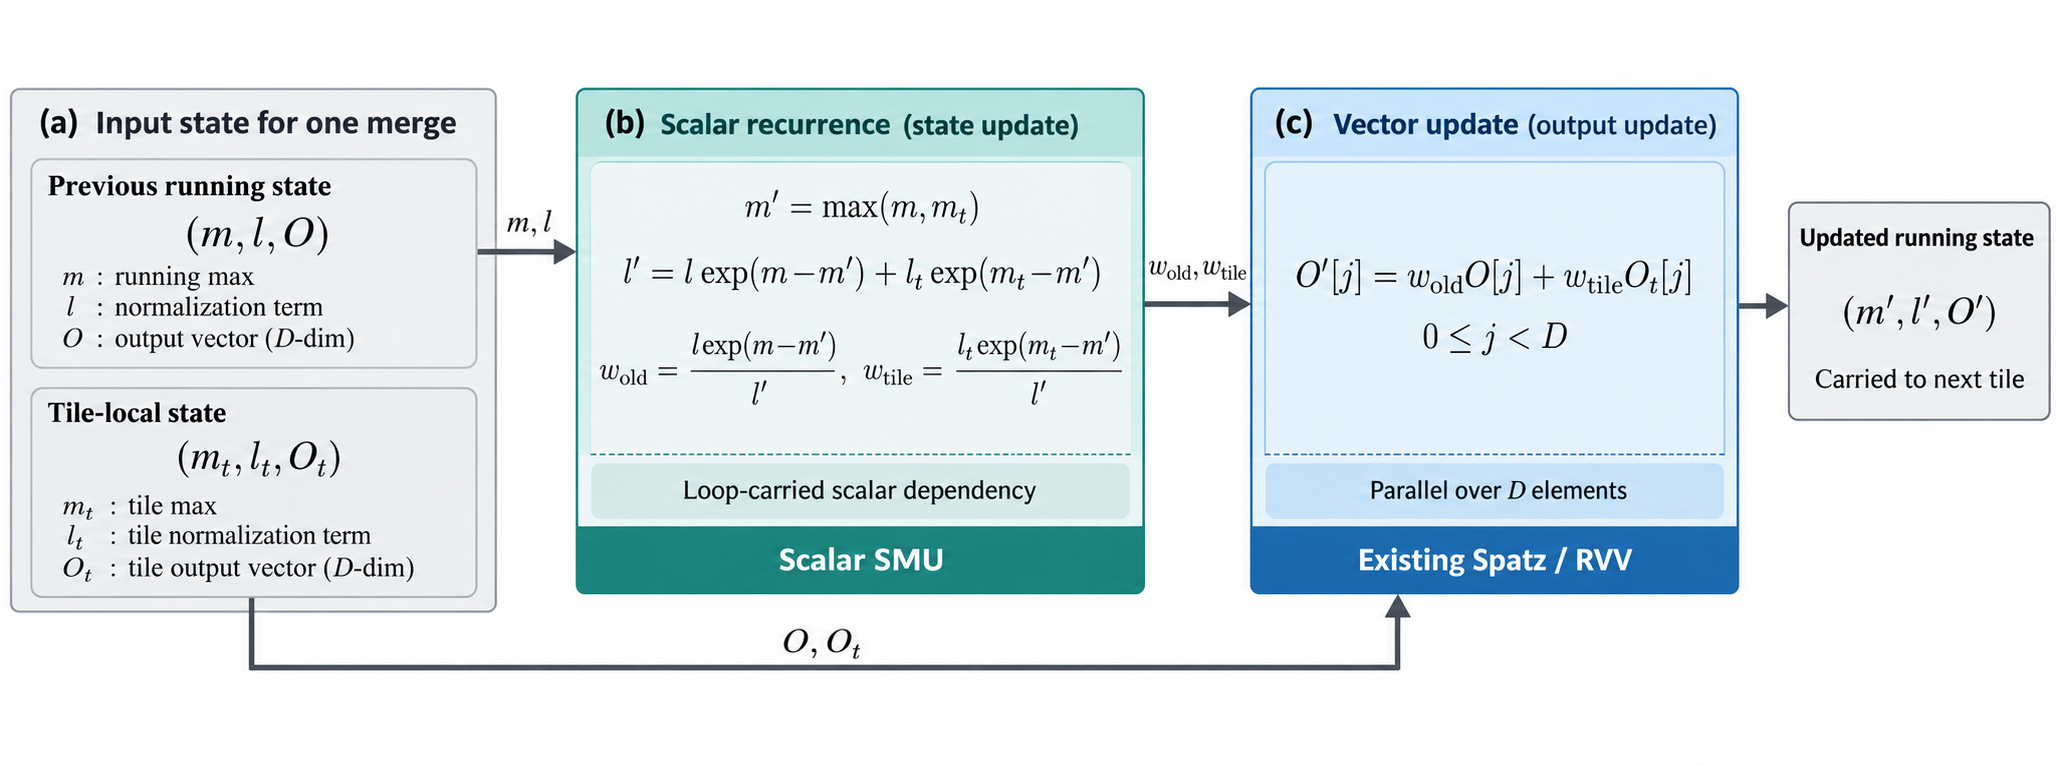
\includegraphics[width=\textwidth,trim=0 58 0 0,clip]{./figure/fig1.png}
\caption{Execution decomposition of a native online-attention merge. The
state-dependent recurrence updates $m$ and $l$ and generates two scalar
rescaling weights. The regular $D$-dimensional output update stays mapped to
the existing Spatz datapath.}
\label{fig:motivation}
\end{figure*}

The recurrence limits intra-merge data parallelism. State carries across tiles,
and maximum selection, exponential rescaling, accumulation, and normalization
form a heterogeneous dependency chain. Its scalar work is independent of $D$,
so increasing $D$ adds no recurrence lanes.

Each output element $j$ obeys the opposite pattern:
\begin{equation}
\label{eq:rvv_o_update}
\mathbf{O}'[j]=w_{\mathrm{old}}\mathbf{O}[j]+w_{\mathrm{tile}}\mathbf{O}_t[j],
\qquad 0\leq j<D,
\end{equation}
All $D$ elements share the same weights and have no inter-element dependency.
The update is a regular floating-point multiply-add loop and maps naturally to
the existing RISC-V Vector (RVV) execution resources. Per query row and per
tile, the recurrence performs a fixed number of scalar operations independent
of $D$, while the output update applies two weighted products to each of the
$D$ elements.

The accelerator therefore targets the recurrence alone. Score generation,
tile-local state construction, and the $D$-dimensional output update stay
programmable, and only the part whose parallelism does not grow with $D$ moves into
hardware. For a configured $N$-row tile merge, the engine repeats this
$O(1)$-in-$D$ recurrence once per row; RVV applies the weights to the $D$
output elements of each row.

\subsection{Design Objectives}
Three objectives follow from these execution characteristics.

The first is selective specialization: dedicate hardware to the recurrence and
reuse Spatz/RVV for the regular output update. That preserves RVV
programmability without duplicating a $D$-wide datapath.

The second is a recurrence unit light enough for cluster integration. Its
stages have different numerical requirements, which Section~III addresses with
stage-aware mixed precision.

The third is a HW/SW interface that lets software configure workload-persistent
context once and invoke recurring merges while hardware tracks the alternating
recurrence state.

In the resulting mapping, a cluster-local mixed-precision Scalar Online-Merge
Unit (SMU) executes the recurrence, the Spatz RISC-V vector datapath performs
the $D$-dimensional output update, and hardware tracks the active A/B selector
for TCDM-resident recurrence state.

\section{Architecture and HW/SW Co-Design}

\subsection{System Overview and HW/SW Partition}
Figure~\ref{fig:system_overview} shows how the design fits into a Spatz vector
cluster~\cite{Spatz2025}. The Snitch scalar core and the Spatz/RVV datapath
share the tightly coupled data memory (TCDM). The cluster-local SMU handles the
Section~II recurrence; Spatz/RVV keeps the regular $D$-dimensional update.

The online-merge (\texttt{OMERGE}) command follows Snitch decode, the per-core
accelerator demultiplexer, cluster issue arbiter, and \texttt{OMERGE} adapter/SMU. The
arbiter records the issuing core, and a response demultiplexer returns
completion to that owner.
Spatz/RVV instructions take the direct vector path. The SMU is an independent
TCDM requester that reads operands and writes scalar state and weights through
the shared memory. The default configuration provides 128~KiB of TCDM in 16
banks.

The integration leaves the Spatz/RVV lanes, floating-point units, vector
register file, and supported instruction semantics untouched, and introduces no
custom RVV instruction. The SMU exchanges scalar state and weights through TCDM, so the RVV routine
applies Eqs.~\eqref{eq:output_update} and \eqref{eq:rvv_o_update} as they
are, with no $D$-wide SMU datapath.

Query, key, and value (Q/K/V) data and working buffers are prepared before the
timed Native Core region. The region excludes allocation, input generation,
diagnostics, Q/K/V loading, and linear projection. It includes score tiles,
local states, first-tile initialization, later merges, RVV updates, and the
final output copy.
The first tile copies $(m_t,l_t,\mathbf{O}_t)$ into the running state. Each later
\texttt{OMERGE} processes all $N$ configured query rows for one score tile. For
each row it reads the active $m,l$ and tile-local $m_t,l_t$, writes $m',l'$ to
the inactive A/B buffers, and stores both weights in TCDM. After all rows
complete, the adapter returns status to the issuing core and commits the A/B
selector only when a successful response is accepted; errors leave it
unchanged. Spatz/RVV then reads the weights and updates each output row, after
which software advances the output pointers. Detailed configuration, invocation,
and selector semantics appear in
Sections~\ref{sec:isa_interface}--\ref{sec:ownership}.

The SMU handles only the scalar recurrence. Score generation, local-state
construction, output addressing and update, first-tile initialization, and the
final copy stay in software or on Spatz/RVV.

\begin{figure}[t]
\centering
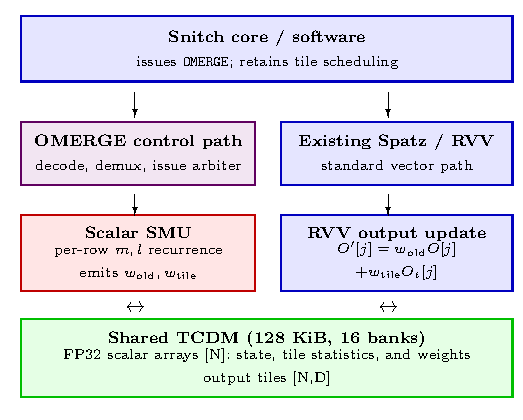
\includegraphics[width=\columnwidth]{./figure/fig2_v4.pdf}
\caption{System integration and HW/SW partition. The Snitch core issues \texttt{OMERGE} through the accelerator decode, demultiplexer, and issue arbiter to the Scalar SMU; the adapter returns completion status to the issuing core. The existing Spatz/RVV path performs the regular output update. Both paths access the shared TCDM for row-wise scalar state, weights, and output tiles.}
\label{fig:system_overview}
\end{figure}

\subsection{Stage-Aware Mixed-Precision SMU}
The SMU assigns precision by stage to accommodate the different numerical
ranges along the recurrence. The assignment is static and shown in
Fig.~\ref{fig:smu_datapath}; input values never select precision at runtime.
What the SMU computes is a stage-quantized approximation of the exact
recurrence in Eq.~\eqref{eq:scalar_merge_recurrence}, not exact FP32
arithmetic. We write $\mathrm{RNE}_{16}(\cdot)$, $\mathrm{FP16}(\cdot)$, and
$\mathrm{Q16.32}(\cdot)$ for conversion to FP16 round-to-nearest-even, FP16,
and the 48-bit unsigned Q16.32 carrier; a hat marks the converted value.
The TCDM interface carries $m$, $m_t$, $l$, and $l_t$ in FP32. The maxima
and their difference use FP16 round-to-nearest-even:
\begin{equation}
\label{eq:fp16_conversions}
\begin{aligned}
\widehat{m} &= \mathrm{RNE}_{16}(m), &
\widehat{m}_t &= \mathrm{RNE}_{16}(m_t),\\
\widehat{m'} &= \max(\widehat{m},\widehat{m}_t), &
\widehat{\Delta}_{\mathrm{old}} &= \mathrm{RNE}_{16}(\widehat{m}-\widehat{m'}),\\
\widehat{\Delta}_{\mathrm{tile}} &= \mathrm{RNE}_{16}(\widehat{m}_t-\widehat{m'}).
\end{aligned}
\end{equation}

The exponential (EXP) stage uses one 256-entry signed Q1.14 lookup table (LUT)
addressed by
\begin{equation}
\label{eq:exp_index}
i(\Delta)=\lfloor(\Delta+8)\cdot32\rfloor,
\qquad \Delta\in[-8,0),
\end{equation}
with bin-center codes and no interpolation. The winning contribution has
$\Delta\geq0$ and bypasses the LUT with exact unity, so equal converted maxima
yield unity on both paths. Contributions with $\Delta\in[-8,0)$ take their
factor from the LUT, where $\Delta=-8$ accesses $\mathrm{LUT}[0]$ and
$\Delta<-8$ gives a zero factor. Denote the factors by
$\widehat{s}_{\mathrm{old}}$ and $\widehat{s}_{\mathrm{tile}}$.

The SMU converts FP32 $l$ and $l_t$ to unsigned Q16.32 carriers, denoted
$\widehat{l}$ and $\widehat{l}_t$, and computes
\begin{equation}
\label{eq:q1632_accumulation}
\widehat{l'}=\widehat{l}\,\widehat{s}_{\mathrm{old}}
            +\widehat{l}_t\,\widehat{s}_{\mathrm{tile}}
\end{equation}
The sum in Eq.~\eqref{eq:q1632_accumulation} remains in the unsigned Q16.32
carrier. The denominator crosses an FP16 RNE boundary before reciprocal
evaluation. For a normalized FP16-rounded denominator
$\widehat{x}=2^{e-127}(1+\mu)$, where $\mu$ is the normalized fractional
mantissa, the reciprocal is approximated by
\begin{equation}
\label{eq:recip_approx}
\begin{aligned}
\frac{1}{\widehat{x}} &\approx 2^{\,127-e}
\Big[L_j+(L_{j+1}-L_j)f_j\Big],\\
j &= \lfloor256\mu\rfloor,\qquad f_j=256\mu-j.
\end{aligned}
\end{equation}
where $L_j$ is the unsigned Q1.15 code for $1/(1+j/256)$ and $f_j$ is carried
in the low 15 mantissa bits. The reciprocal value from
Eq.~\eqref{eq:recip_approx} scales each numerator.
Each scaled numerator
also crosses the FP16 RNE boundary and returns to Q16.32 before weight
computation. One shared 48$\times$16 multiplier produces the old and tile
weights sequentially. The reciprocal-LUT path is selected by the
\texttt{ONLINE\_MERGE\_MIXED\_RECIPROCAL} build definition; its provenance is
reported with the evaluation results.

The datapath handles denominators that remain positive and finite after FP16
conversion, and fixed-point intermediates stay within the Q16.32 range.
Directed model tests cover zero numerators, subnormal denominators, and the
largest finite FP16 denominator. Stage quantization error comes from EXP
truncation, LUT quantization, and FP16 rounding.

The engine writes $\widehat{m^{\prime}}$ and $\widehat{l^{\prime}}$ back to TCDM in FP32: the
maximum carries FP16 rounding and the normalizer carries the Q16.32
accumulation. Merge weights become
$w=\mathrm{FP32}(\mathrm{FP16}(\widehat{w}))$ through the conversions of
Eq.~\eqref{eq:fp16_conversions} and are consumed by the unchanged FP32
Spatz/RVV update. The memory interface is FP32, the internal recurrence is
stage-wise FP16 and fixed point, and all precision assignments are fixed at
design time.

\begin{figure}[t]
\centering
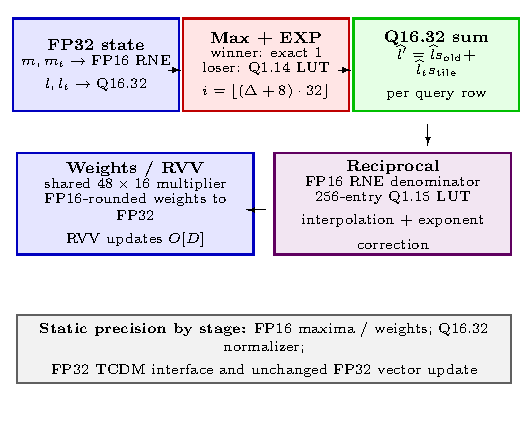
\includegraphics[width=\columnwidth]{./figure/fig3_v4.pdf}
\caption{Stage-aware mixed-precision Scalar SMU datapath. The diagram shows per-row FP32 state, FP16-RNE maxima and reciprocal boundary, Q16.32 normalization, direct-bin EXP lookup, interpolated reciprocal correction, and FP16-to-FP32 merge weights for the unchanged RVV output update.}
\label{fig:smu_datapath}
\end{figure}

\subsection{RISC-V Instruction Interface}
\label{sec:isa_interface}
The programming model separates persistent context setup from recurring
execution. Both operations use the RISC-V custom-2 opcode space reserved for
implementation-specific extensions~\cite{riscv_unprivileged} and enter the
existing Snitch accelerator request path in the Spatz cluster
~\cite{Spatz2025}. Their encodings and architectural effects are listed in
Table~\ref{tab:isa_interface}, with exact decoder patterns in
Table~\ref{tab:encodings}. Neither instruction changes the RVV encoding or
the semantics of supported vector instructions.

\begin{table*}[t]
\centering
\caption{Custom-2 instruction formats and architectural effects.}
\label{tab:isa_interface}
\scriptsize
\setlength{\tabcolsep}{2pt}
\begin{tabular}{@{}l p{4.6cm} p{3.8cm} p{7.2cm}@{}}
\toprule
Instruction & Encoding fields & Register and immediate fields & Architectural effect \\
\midrule
\texttt{OMERGE} &
R-type; opcode \texttt{0x5B}; funct7 \texttt{0000011}; funct3 \texttt{000} &
\texttt{rs1=rs2=x0}; \texttt{rd} is the status destination &
Processes all configured $N$ rows for one score tile, reads and writes each
row's scalar recurrence state through TCDM, stores the two weights, and returns
completion status. \\
\addlinespace
\texttt{OMCFG} &
I-type-like; opcode \texttt{0x5B}; funct3 \texttt{001}; \texttt{imm12=cfg\_id} &
\texttt{rs1} supplies the value; \texttt{rd=x0} &
Writes one persistent context field or issues the separate INIT commit
operation. It starts no recurrence and returns no register result. \\
\bottomrule
\end{tabular}
\end{table*}

\begin{table}[t]
\centering
\caption{Exact decoder patterns for the two custom-2 commands. The adapter recognizes a word when its bitwise AND with the mask equals the match value.}
\label{tab:encodings}
\scriptsize
\setlength{\tabcolsep}{4pt}
\begin{tabular}{@{}l L{6.2cm}@{}}
\toprule
Command & Mask, match, and machine word \\
\midrule
\texttt{OMERGE} & mask \texttt{0xFFFFF07F}, match \texttt{0x0600005B}, word
\texttt{0x0600005B | (rd << 7)}; \texttt{instruction[11:7]} encodes \texttt{rd},
the completion-status destination, while \texttt{rs1=rs2=x0}. \\
\addlinespace
\texttt{OMCFG} & mask \texttt{0x00007FFF}, match \texttt{0x0000105B}, word
\texttt{(cfg\_id << 20) | (rs1 << 15) | 0x0000105B}; the 12-bit
\texttt{cfg\_id} occupies bits [31:20] and \texttt{rs1} supplies the field
value in bits [19:15], with \texttt{rd=x0}. \\
\bottomrule
\end{tabular}
\end{table}

Table~\ref{tab:encodings} gives the exact decoder masks, match values, and
machine-word expressions. The fixed function bits separate the recurring
command from the configuration namespace while keeping both operations in
custom-2.

\texttt{OMERGE} is a scalar recurrence command, not a vector operation. Its
\texttt{rs1} and \texttt{rs2} fields both name \texttt{x0}. Each command
applies the scalar recurrence to all $N$ configured rows of one score tile,
reading $m$, $l$, $m_t$, and $l_t$ and writing $m'$, $l'$, and the two
rescaling weights through TCDM. No $D$-dimensional output data crosses the
instruction interface. The adapter
fixes the engine to Mixed Scalar mode, matching the arithmetic used by the
MMIO-controlled SMU path; the existing RVV routine performs the output update.

The \texttt{rd} field names the status destination. Software must use a
nonzero destination to inspect the returned status; \texttt{rd=x0} discards
the register write. On issue, Snitch reserves that destination in its
accelerator scoreboard and forwards the instruction and
request identifier through the per-core accelerator demultiplexer and cluster
issue arbiter. The adapter permits one outstanding command and follows
\texttt{IDLE}, \texttt{START}, \texttt{WAIT}, and \texttt{RESP}. In
\texttt{WAIT}, it waits for the SMU to report DONE or ERROR. In
\texttt{RESP}, the response path returns the request identifier and status to
the issuing core; accepting that response writes \texttt{rd} and clears its
pending scoreboard entry. A zero status denotes success and a nonzero status
denotes an error. The instruction is therefore complete to software only
after the core accepts the accelerator response.

The recurring timing comparison covers this complete path: issue, SMU
execution and busy time, response commit, and status consumption. The separate
\texttt{OMERGE} interface comparison holds the SMU arithmetic and RVV update
constant while changing how each non-first-tile recurrence is invoked.

\subsection{Runtime-Configurable Context with \texttt{OMCFG}}
Addresses and workload parameters need to persist across a sequence of tile
merges. Rewriting them around every recurrence would put setup traffic back in
the steady-state path. \texttt{OMCFG} writes workload-persistent context once; each later score tile
uses one \texttt{OMERGE} invocation to process all configured query rows.

\begin{figure*}[t]
\centering
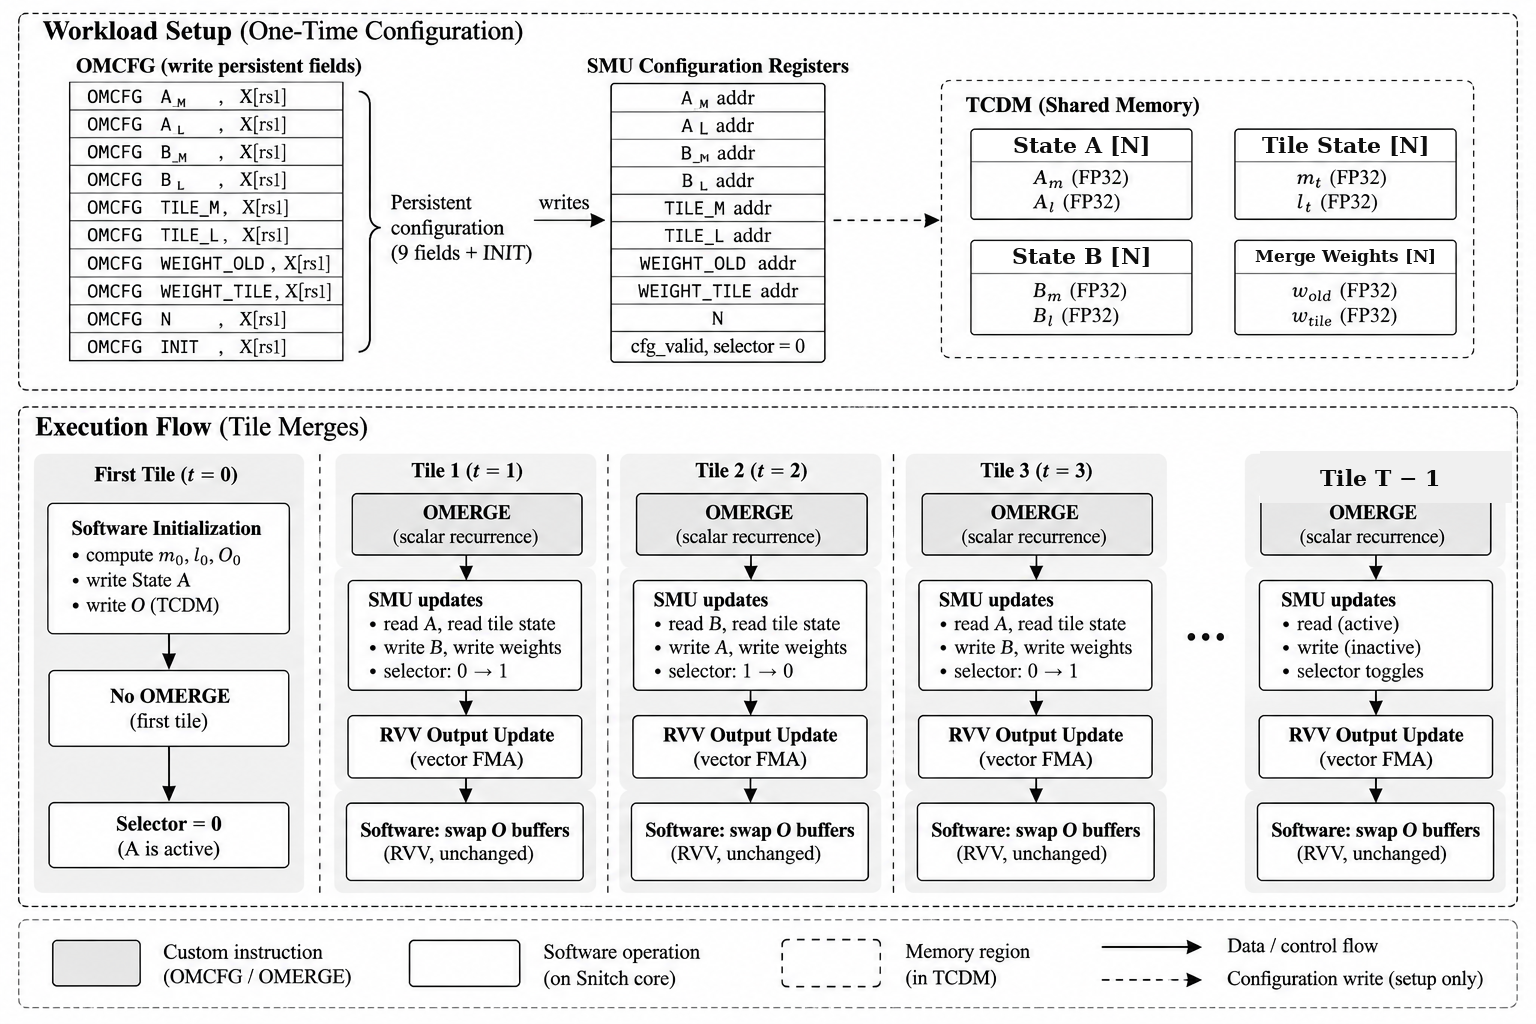
\includegraphics[width=\textwidth]{./figure/fig4_v4.png}
\caption{\texttt{OMCFG}/\texttt{OMERGE} programming model. One-time
\texttt{OMCFG} writes establish persistent scalar context and reset the
selector. Each later score tile uses one \texttt{OMERGE} command to process
the configured $N$ query rows before the unchanged RVV output update. With
tile size $B=4$, a workload of $N$ rows has $T=N/B$ tiles, and the final tile
is $T-1$. The dashed setup path writes context addresses, not TCDM data.
Hardware toggles only the A/B scalar-state selector; software swaps output
buffers. The selector changes after the issuing core accepts a successful
response.}
\label{fig:programming_model}
\end{figure*}

Figure~\ref{fig:programming_model} places the four ownership classes on the
execution timeline: \texttt{OMCFG} establishes persistent context, \texttt{OMERGE} advances the
scalar state, hardware toggles the selector after successful completion, and
software updates the output-buffer pointers.

\texttt{OMCFG} uses the same custom-2 opcode as \texttt{OMERGE} and selects
funct3 \texttt{001}. The I-type-like encoding places a 12-bit configuration
identifier in \texttt{imm12} and the value in \texttt{rs1}; \texttt{rd} is
fixed to \texttt{x0}. This creates no destination scoreboard entry and
returns no writeback payload. The adapter accepts a configuration command
only while the adapter and SMU engine are idle. The immediate selects a
field; it does not carry the field value.

IDs \texttt{0x000}--\texttt{0x008} write nine required fields. They specify the physical TCDM base addresses for the two running-state pairs, tile-local $m_t/l_t$, the two weight arrays, and query-row count $N$. ID \texttt{0x009} selects the separate CTRL/INIT operation; its value bit~0 commits a complete context and resets the selector. Table~\ref{tab:omcfg_map} lists the mapping and its boundary. Each configured address is the base of a per-row FP32 array; \texttt{scalar\_addr(base,row)=base+(row<<2)} places row $r$ at byte offset $4r$.

\begin{table*}[t]
\centering
\caption{\texttt{OMCFG} configuration-ID map. IDs 0--8 are the required
context fields; ID 9 is the separate INIT control operation.}
\label{tab:omcfg_map}
\scriptsize
\setlength{\tabcolsep}{3pt}
\begin{tabular}{@{}c l p{6.3cm} p{7.0cm}@{}}
\toprule
\texttt{cfg\_id} & Field & Value or address & Purpose and write semantics \\
\midrule
\texttt{0x000} & \texttt{A\_M} & TCDM address & Per-row running maximum array in state buffer A \\
\texttt{0x001} & \texttt{A\_L} & TCDM address & Per-row running normalizer array in state buffer A \\
\texttt{0x002} & \texttt{B\_M} & TCDM address & Per-row running maximum array in state buffer B \\
\texttt{0x003} & \texttt{B\_L} & TCDM address & Per-row running normalizer array in state buffer B \\
\texttt{0x004} & \texttt{TILE\_M} & TCDM address & Per-row tile-local maximum array $m_t$ \\
\texttt{0x005} & \texttt{TILE\_L} & TCDM address & Per-row tile-local normalizer array $l_t$ \\
\texttt{0x006} & \texttt{WEIGHT\_OLD} & TCDM address & Base of per-row $w_{\mathrm{old}}$ array \\
\texttt{0x007} & \texttt{WEIGHT\_TILE} & TCDM address & Base of per-row $w_{\mathrm{tile}}$ array \\
\texttt{0x008} & \texttt{N} & Query-row count & Rows processed by each \texttt{OMERGE} invocation \\
\texttt{0x009} & \texttt{CTRL/INIT} & Bit~0 = 1 & Commit all required fields and reset the A/B selector \\
\texttt{0x00A--0xFFF} & Reserved & No register write & Unsupported IDs invalidate readiness until a complete INIT \\
\bottomrule
\end{tabular}
\end{table*}

The nine required fields share the canonical generated registers with the
legacy MMIO interface. An \texttt{OMCFG} write updates the same register as
MMIO, so an MMIO read observes the written value. The adapter tracks writes
with a \texttt{9'h1FF} mask and marks the context dirty. INIT with bit~0 set
commits only when all nine required bits are present; success sets
\texttt{cfg\_valid} and resets the selector to zero. INIT with bit~0 clear
does not commit. Rewriting a required field makes another complete INIT
necessary before the next merge.

\texttt{OMCFG} configures scalar state, tile-local statistics, weight
addresses, and the query-row count. The output dimension $D$, tile size,
output-vector addresses, and stride remain software and RVV parameters: the
adapter fixes Mixed Scalar mode and supplies the corresponding internal fields
as $D=1$ and zero stride. A reserved ID performs no register write and leaves
the context pending initialization until software issues a complete INIT. The
interface evaluation therefore separates one-time setup from recurring
invocation and from the broader Native Core window.

\subsection{Invocation Sequence and State Ownership}
\label{sec:ownership}
The programmed addresses name two physical running-state buffers. A
one-bit hardware selector identifies which pair supplies the current scalar
state and which pair receives the next state, avoiding per-merge address
updates in software. Figure~\ref{fig:programming_model} shows the lifetime:
software initializes the first tile and output state, writes the nine
required fields, commits INIT, then issues one \texttt{OMERGE} for each later
tile. After a successful response, the existing RVV routine updates the
output and software swaps its output-buffer pointers.

The selector operates on two TCDM-resident buffer pairs
$A=(A_m,A_l)$ and $B=(B_m,B_l)$, each holding one FP32 maximum and one FP32
normalizer per query row $0\leq r<N$.

Selector zero selects $A$ as the source and $B$ as the destination. Selector
one selects $B$ as the source and $A$ as the destination. The selector changes
the physical \texttt{m/l} addresses supplied to the SMU. The buffers stay in
TCDM and retain their contents.

Software handles the first tile as initialization. It writes the initial
running scalar state into $A$ and initializes the output buffer in software,
so no \texttt{OMERGE} runs for that tile. A complete INIT
leaves the selector at zero. The first later merge reads $A$ and writes $B$; subsequent merges alternate the
direction.

The adapter commits a selector transition only when the issuing core accepts a
zero-error accelerator response. Issue and SMU start leave the selector
unchanged. An incomplete or dirty context returns a nonzero status without
asserting engine start. An SMU error also returns a nonzero status. Both cases
leave the selector at its previous value, so a failed command cannot redirect
the next successful merge.

The selector owns only the per-row scalar $m/l$ state. Software continues to maintain
the two $D$-dimensional output-buffer pointers, and the unchanged RVV routine
performs the output update after each successful recurrence. Software also owns
tile addresses and output pointers.
The evaluated contract uses one controlling core and one active context.
Hardware owns the per-row $m/l$ A/B selector; software owns tile addresses and
the two $D$-dimensional output-buffer pointers. After each successful
recurrence, software consumes the returned status, runs the RVV update, and
swaps the output-buffer pointers.

\section{Evaluation}

\subsection{Experimental Setup and Measurement Scope}
Performance results come from cycle-level simulation of the Spatz RISC-V vector
cluster. The Verilated model uses Verilator 5.034 and the default cluster
configuration with 128~KiB of 16-bank TCDM. Cycle counters bracket each
measured stage explicitly, and every matched comparison runs on the same frozen
cluster configuration and software toolchain.

N8/D32 and N16/D64 are the two anchor workloads. N24/D64 and N16/D128 test
whether the observed behavior survives a change in sequence length or output
dimension. All native-attention cases use tile size $B=4$ and seed one. The
first tile initializes the running state directly and needs no merge. Each
query row therefore has $T-1$ later-tile merges: one at N8/D32, three at
N16/D64, five at N24/D64, and three at N16/D128. Each later score tile issues
one \texttt{OMERGE}, which processes all configured $N$ rows.

The design accelerates only part of native online attention, so we report three
timing scopes. The B2R software \emph{recurrence} window covers the scalar
state-dependent update that produces $m'$, $l'$, $w_{\mathrm{old}}$, and
$w_{\mathrm{tile}}$. For the matched MMIO-controlled SMU path, the reported
recurrence window also includes per-merge register programming, clear/start,
BUSY/DONE polling, and SMU execution. It therefore measures the complete
recurrence invocation, including control and engine-busy time, rather than
arithmetic-only latency. The \emph{merge} window adds the corresponding RVV
output update and the merge-side orchestration. The \emph{Native Core} window
adds score-tile computation, tile-local state construction, first-tile handling,
all later merges, and the final output handling. Allocation, input generation,
diagnostics, Q/K/V loading, and linear projection stay outside all three.

The comparisons form independent matched families. The arithmetic-offload
family compares a scalar-software recurrence plus RVV (B2R) with the
MMIO-controlled Mixed Scalar SMU plus the same RVV update. The recurring-
interface family holds SMU arithmetic and RVV common and compares per-merge
MMIO control with \texttt{OMERGE}. The configuration family holds
\texttt{OMERGE} common and compares one-time MMIO configuration with
\texttt{OMCFG}. Full SMU appears only in the separate ablation.

Each family uses its own matched baseline and frozen implementation. B2R
implements the same mathematical recurrence and shares the RVV routine, but the
two paths use different internal numerical formats, so the recurrence ratio
reflects hardware specialization together with the stage precision assignment.
The simulation uses fixed inputs, and each interface family takes one formal
measurement per path and shape. Speedups are cycle-count ratios.

\subsection{Native Online Attention Performance}
\label{sec:native_performance}
The native comparison holds the output update constant to measure recurrence
offload. B2R is the matched software baseline: it executes the recurrence in
scalar software and shares the SMU path's RVV output routine.
Figure~\ref{fig:native_performance} summarizes the three timing scopes.

\begin{figure*}[t]
\centering
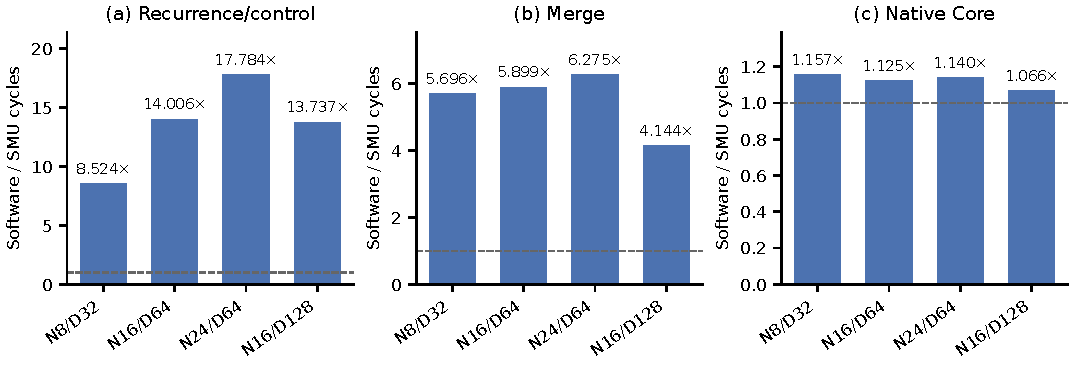
\includegraphics[width=\textwidth]{./figure/fig5.pdf}
\caption{Native online-attention speedup across recurrence, merge, and Native
Core measurement scopes. The MMIO-controlled SMU recurrence window includes
per-merge configuration, clear/start, polling, and SMU execution. Ratios use
matched software and SMU cycle counts, tile size four, and seed one. The three
panels use separate vertical scales.}
\label{fig:native_performance}
\end{figure*}

At N8/D32 the recurrence falls from 12,368 to 1,451 cycles, an 8.524$\times$
speedup. The merge window falls from 13,204 to 2,318 cycles, or 5.696$\times$.
Native Core cycles drop from 85,262 to 73,706, a 1.157$\times$ speedup and a
13.554\% cycle reduction.

At N16/D64 the recurrence falls from 68,994 to 4,926 cycles, or 14.006$\times$.
The merge window falls from 77,037 to 13,060 cycles, 5.899$\times$. Native Core
drops from 571,374 to 507,918 cycles, a 1.125$\times$ speedup and an 11.106\%
reduction.

N24/D64 reaches 17.784$\times$ at
the recurrence scope, 6.275$\times$ at the merge scope, and 1.140$\times$ at
the Native Core scope. N16/D128 reaches 13.737$\times$, 4.144$\times$, and
1.066$\times$ at those same three scopes. Across all four workloads the
measured ranges are 8.524--17.784$\times$ for recurrence,
4.144--6.275$\times$ for merge, and 1.066--1.157$\times$ for Native Core.

As the scope widens, score construction, tile-local state generation, and the
regular vector output update enter the total, and their share grows.
The recurrence, merge, and Native Core ratios therefore decrease in that order.

\subsection{Numerical Fidelity and Standalone SMU Cost}
The stage-aware mixed-precision SMU agrees closely with the matched B2R
software recurrence and reduces standalone mapped area. Across the four
native-attention workloads, the MAE is $2.8\times10^{-4}$ to
$5.6\times10^{-4}$ and the relative error is 0.49\% to 0.71\%. No output is
nonfinite in these cases.

\begin{table*}[t]
\centering
\caption{Numerical agreement with the B2R software recurrence and standalone
SMU area. Area is reported in Nangate45 library cell-area units.}
\label{tab:numerical_ppa}
\scriptsize
\setlength{\tabcolsep}{4pt}
\begin{tabular}{@{}lcc@{}}
\toprule
\multicolumn{3}{@{}l@{}}{\textit{(a) Agreement with B2R software outputs}} \\
Shape & MAE & Relative error \\
\midrule
N8/D32 & $2.79\times10^{-4}$ & 0.49\% \\
N16/D64 & $4.67\times10^{-4}$ & 0.71\% \\
N24/D64 & $3.74\times10^{-4}$ & 0.61\% \\
N16/D128 & $5.63\times10^{-4}$ & 0.52\% \\
\midrule
\multicolumn{3}{@{}l@{}}{\textit{(b) Standalone synthesis}} \\
Design & Mapped area (library units) & Area reduction vs. Legacy \\
\midrule
Legacy Scalar & 72,399 & n/a \\
Mixed+Division & 52,000 & 28.2\% \\
Mixed+Reciprocal & 52,408 & 27.6\% \\
\bottomrule
\end{tabular}
\end{table*}

Table~\ref{tab:numerical_ppa}(a) compares the native cases with B2R software
outputs; both metrics are computed in float64 from the stored FP32 results, and
the relative error is $\sum|\Delta|/\sum|O|$. Sweeping all 31,743 positive
finite FP16 denominators exhaustively gives a maximum reciprocal relative error
of $6.70\times10^{-5}$. The host-model scan covers random-score and
single-head Q/K/V cases, lengths 128, 256, 512, and 1024, and dimensions 64 and
128 (16 combinations), with tile size 32 and base seed 20260823; it is distinct
from the tile-four RTL native-performance experiments. Across the reciprocal-LUT
parameter scan, replacing division with the reciprocal LUT gives a maximum
relative error of 0.11\%, and the optimized implementation against an FP32
reference gives a maximum relative error of 1.5\%.

Stage-aware precision is measured with matched standalone Yosys/ABC synthesis
against the Nangate45 typical library. Replacing the Legacy arithmetic with
mixed precision while
keeping division cuts mapped area from 72,399 to 52,000 units, a 28.2\%
reduction. The final reciprocal implementation occupies 52,408 units, which is
27.6\% below Legacy and 0.8\% above Mixed+Division.

\subsection{HW/SW Partition Ablation}
\label{sec:ablation}
The final architecture keeps the $D$-dimensional output update on RVV and omits
a dedicated vector datapath in the SMU. We examine this choice with a separate
Full SMU/A2 experiment, which measures merge microkernel cycles: both designs
come from the same ablation implementation, while the mixed-precision synthesis
results of Table~\ref{tab:numerical_ppa}(b) come from a separate
implementation.

There, the selective design combines scalar recurrence offload with the RVV
output update, and Full SMU additionally moves the dimension-dependent output
update into the accelerator. Standalone area rises from 77,103 to 114,713
library units, a 48.8\% increase.

\begin{table}[t]
\centering
\caption{Selective-versus-full-offload ablation on merge microkernel cycles.
The cycle window and implementation are common within each row.}
\label{tab:full_smu_ablation}
\scriptsize
\setlength{\tabcolsep}{4pt}
\begin{tabular}{@{}lrrr@{}}
\toprule
Shape & Selective & Full SMU & Full/Selective \\
\midrule
N12/D64  & 4,128  & 7,704  & 1.866$\times$ \\
N32/D128 & 12,866 & 34,728 & 2.699$\times$ \\
N40/D128 & 15,733 & 43,206 & 2.746$\times$ \\
\bottomrule
\end{tabular}
\end{table}

Full SMU costs more cycles than the selective design in all three matched
workloads. Together with the area comparison, these results support keeping the
regular $D$-dimensional output update on the RVV datapath instead of
duplicating it inside the SMU.

\subsection{RISC-V Instruction-Interface Evaluation}
\label{sec:isa_evaluation}
The ISA interface is evaluated in two stages: recurring per-merge invocation
first, then one-time workload configuration with \texttt{OMERGE} held common.

A1-MMIO and A1-ISA/\texttt{OMERGE} use the same Mixed Scalar SMU arithmetic, RVV output
routine, workload, tile size, and numerical semantics. They differ only in how
each non-first-tile recurrence is triggered. Table~\ref{tab:isa_results}(a)
reports the matched windows in cycles for both anchors.

The inclusive recurrence/control window contains issue and control activity, SMU
execution and busy time, response commit, and status consumption, so its
reduction measures more than dispatch latency. Most of that window is SMU busy
time, which both paths pay at equal or nearly equal cost. Subtracting it isolates the control activity around
the recurrence: 1,261 cycles fall to 40 at N8/D32 and 3,577 fall to 81 at
N16/D64. Widening the scope adds work the interface does not touch, so the
reported reduction falls to 41.695\% and 21.954\%
at the merge scope, and to 0.841\% and 0.448\% when the one-time ISA setup
enters the Native Core window.

With \texttt{OMERGE} held common, we compare MMIO-config+\texttt{OMERGE} against
\texttt{OMCFG}-config+\texttt{OMERGE}. Both variants execute the same \texttt{OMERGE}-based Native Core.
They differ only in the transport of nine configuration fields and one INIT
operation before core execution. For N8/D32, setup decreases from 991 to 659
cycles, a 33.50\% reduction. For N16/D64, it decreases from 986 to 632 cycles,
a 35.90\% reduction. Native Core execution is identical for N8/D32 and differs
by only 12 cycles for N16/D64; the corresponding setup-inclusive totals fall by
0.451\% and 0.067\%, respectively. Table~\ref{tab:isa_results} summarizes
both comparisons.

\begin{table}[t]
\centering
\caption{ISA interface evaluation. In (a), both paths use the same Mixed
Scalar SMU arithmetic and RVV routine, so SMU busy cycles inside the recurrence
and merge windows cancel or nearly cancel (N16/D64 differs by 4 cycles). The
control row subtracts the common busy cycles and leaves launch, poll, and
commit activity.}
\label{tab:isa_results}
\scriptsize
\setlength{\tabcolsep}{2pt}
\begin{tabular}{@{}llrrr@{}}
\toprule
\multicolumn{5}{@{}l@{}}{\textit{(a) \texttt{OMERGE} per-merge effect (cycles)}} \\
Shape & Window & MMIO & \texttt{OMERGE} & Reduction \\
\midrule
N8/D32 & Ctrl. excl. busy & 1,261 & 40 & 96.828\% \\
       & Rec./Ctrl. & 2,069 & 848 & 59.014\% \\
       & Merge & 2,926 & 1,706 & 41.695\% \\
       & Setup-incl. Core & 74,392 & 73,766 & 0.841\% \\
\addlinespace
N16/D64 & Ctrl. excl. busy & 3,577 & 81 & 97.736\% \\
        & Rec./Ctrl. & 8,429 & 4,929 & 41.523\% \\
        & Merge & 16,548 & 12,915 & 21.954\% \\
        & Setup-incl. Core & 510,991 & 508,702 & 0.448\% \\
\midrule
\multicolumn{5}{@{}l@{}}{\textit{(b) \texttt{OMCFG} setup effect}} \\
Shape & \shortstack{MMIO\\ setup} & \shortstack{\texttt{OMCFG}\\ setup} &
\shortstack{Setup\\ reduction} & \shortstack{Native Core\\ $\Delta$} \\
\midrule
N8/D32 & 991 & 659 & 33.50\% & 0 \\
N16/D64 & 986 & 632 & 35.90\% & +12 \\
\bottomrule
\end{tabular}
\end{table}

Both interface comparisons preserve functional behavior. The \texttt{OMERGE} and
MMIO-controlled paths produce bit-identical final outputs for both anchor
workloads. N8/D32 issues one \texttt{OMERGE} and N16/D64 issues three, matching the
expected number of non-first-tile merges and selector transitions; each command
processes all configured query rows. The final
output hashes are \texttt{0x9c7cdedc} for N8/D32 and \texttt{0xfd0d2cff} for
N16/D64. The matched outputs have zero pairwise MAE and zero stable relative
error, and no nonfinite values.

Both configuration routines are present in each binary. A data-resident
\texttt{volatile} path selector has a different initial value in the two
builds and selects MMIO or OMCFG at runtime. Consequently, the
MMIO-config and \texttt{OMCFG}-config binaries have byte-identical \texttt{.text}
within each workload and produce word-for-word identical final outputs. They
also establish identical persistent configuration state after INIT, including
all nine fields and selector zero. The \texttt{OMCFG} gain is therefore
concentrated in context setup.

\subsection{Explicit-P Negative Control}
The final experiment tests the SMU as a general replacement for row-wise
Softmax in an explicit probability-matrix dataflow. The surrounding
quantized-attention path is held fixed; only the explicit-P software Softmax
backend is swapped for the Mixed SMU backend.

For N8/D32, Mixed SMU increases the explicit-P Softmax window from 12,502 to
14,812 cycles, making it 18.477\% slower than software. For N16/D64, the
window changes from 48,595 to 48,534 cycles, a 0.126\% improvement. The wider
attention windows remain slightly slower with the SMU in both cases.

The five-stage Attention Total changes from 839,111 to 841,597 cycles for
N8/D32, a 0.296\% increase, and from 6,767,387 to 6,768,406 cycles for
N16/D64, a 0.015\% increase. The complete Mixed Softmax window includes $P$
initialization, SMU launch and polling, the RVV probability update, and
swap/clear orchestration. The five-stage Attention Total sums arithmetic terms;
it does not come from an independent timing counter.

Row-wise normalization offload therefore returns no overall benefit through a
flow that also contains $P$ initialization, control, and the RVV probability
update. Together with the native results of
Section~\ref{sec:native_performance}, this contrast locates the benefit of the
partition in the recurrence itself rather than in per-row normalization.

\section{Discussion}
\label{sec:discussion}

\subsection{The gain follows the chosen execution boundary}
The measured benefit is largest at the recurrence boundary and narrows as the
window includes work left on the programmable path. Score-tile computation and
the regular $D$-element output update remain outside the scalar accelerator;
the Native Core result therefore reflects this partition's effect on the
measured kernel, with Q/K/V loading and linear projections excluded.

Four native workloads gain Native Core cycles, while the two explicit-P cases
lose a small number. In the explicit-P flow, row-wise normalization is a small
fraction of a stage that also contains $P$ initialization, control, and the RVV
probability update. The benefit of offloading the scalar recurrence therefore
tracks the share of the target kernel that the recurrence occupies.

\subsection{The instruction interface exposes the partition to software}
Software writes the nine supported context fields with \texttt{OMCFG} and
commits readiness, then invokes \texttt{OMERGE} for each later score tile.
Hardware processes all configured query rows and tracks the alternating
scalar-state selector; software retains tile scheduling, output-buffer
pointers, and RVV execution. The core's accelerator path exposes this stateful
operation without a custom vector instruction or a duplicated output datapath.

\texttt{OMERGE} shortens the recurrence/control window by 41.5--59.0\% on the
two anchors, and \texttt{OMCFG} shortens one-time configuration by
33.5--35.9\%, so the interface lowers both the per-merge invocation cost and
the context setup cost. Setup-inclusive totals change by 0.451\% and 0.067\%,
which places these gains on the control plane that complements the selective
dataflow.

VEXP provides exponentiation through scalar and packed-SIMD instructions.
\texttt{OMERGE} instead works at the granularity of one tile merge, grouping
maximum update, exponential rescaling, normalization, and state writeback into
a single stateful invocation; \texttt{OMCFG} supplies the configuration
context that persists across tiles, and hardware selects the alternating
scalar-state buffer.

\section{Comparison with Prior Work}
\label{sec:comparison}

Table~\ref{tab:related_work} places this work among representative RISC-V and
AI acceleration approaches; the subsections below give the detail behind each
row.

\begin{table*}[t]
\centering
\caption{Positioning of representative RISC-V and AI acceleration approaches.}
\label{tab:related_work}
\scriptsize
\setlength{\tabcolsep}{2.2pt}
\renewcommand{\arraystretch}{0.94}
\begin{tabular}{@{}L{2.0cm}L{9.0cm}L{5.8cm}@{}}
\toprule
Work & Hardware path and vector relation & Reported result \\
\midrule
VEXP \cite{wang2025vexp} &
Snitch FPU with custom scalar/packed \texttt{FEXP}/\texttt{VFEXP} for BF16
exponentiation &
162.7$\times$ lower Softmax latency; 8.2$\times$ FlashAttention-2 speedup \\
\addlinespace[1pt]
SoftEx \cite{belano2025softex} &
RISC-V cluster HWPE accelerates Softmax/GELU through control and streaming
interfaces &
10.8$\times$ Softmax speedup; 1.58$\times$ end-to-end ViT throughput \\
\addlinespace[1pt]
TOP-V \cite{chen2026topv} &
Ara vector processor with custom \texttt{VTOPK} sorting instruction &
5.24$\times$ over RVV-based sorting \\
\addlinespace[1pt]
RedMulE \cite{tortorella2023redmule} &
Cluster-local HWPE-style GEMM engine sharing cluster memory &
15$\times$ GEMM; up to 62$\times$ GEMM-Op over software \\
\addlinespace[1pt]
Gemmini \cite{genc2021gemmini} &
RoCC-attached systolic array with a full software stack &
Full-stack DNN evaluation; orders-of-magnitude over CPU baselines \\
\addlinespace[1pt]
Deeploy \cite{scherer2024deeploy} &
Compiler maps SLM execution across RV32 cores, ML extensions, and an NPU &
340 token/s at 490~$\mu$J/token (TinyStories SLM) \\
\addlinespace[1pt]
\textbf{This work} &
Cluster-local Scalar SMU with \texttt{OMCFG}/\texttt{OMERGE} specializes the
recurrence; Spatz/RVV retains the output update &
Up to 17.784$\times$ recurrence, 6.275$\times$ merge, and 1.157$\times$ Native Core (MMIO-controlled SMU) over the B2R software baseline \\
\bottomrule
\end{tabular}
\end{table*}

\subsection{Softmax and Nonlinear Acceleration}

Once matrix multiplication is well optimized, nonlinear operators such as
exponentiation, Softmax, and GELU become the bottleneck in Transformer
workloads. Prior work attacks this at several granularities, from arithmetic
ISA extensions and low-cost reconfigurable nonlinear
cores~\cite{li2020nonlinear,wu2025nonlinear} to dedicated nonlinear
accelerators.

VEXP puts an approximate BFloat16 exponential unit inside the floating-point
unit of Snitch RISC-V cores and exposes it through scalar \texttt{FEXP} and
packed-SIMD \texttt{VFEXP} instructions \cite{wang2025vexp}. Its Softmax kernel
pairs that exponential with the existing Snitch execution mechanisms, and
reports up to 162.7$\times$ lower Softmax latency and an 8.2$\times$ gain for
FlashAttention-2 in the GPT-2 configuration. VEXP is a fine-grained approach:
it adds the costly nonlinear primitive to the programmable datapath.

SoftEx takes the other route and accelerates the whole nonlinear operator in
dedicated BFloat16 hardware \cite{belano2025softex}. Its datapath covers
approximate exponentiation, accumulation, inversion, and normalization, and
sits in a RISC-V cluster next to a matrix engine. The extended design also
supports GELU and reports up to 10.8$\times$ Softmax acceleration, which shows
what nonlinear hardware beside an already accelerated matrix path can buy.

Our comparison focuses on a different exposed interface: persistent normalized
state and per-merge control. Online attention carries that scalar state across
tiles and calls the SMU once per merge, while RVV performs the
$D$-dimensional output update.

\subsection{RISC-V Domain-Specific Acceleration}

RISC-V's extensibility lets domain-specific hardware stay under software
control without a separate programming model. Systems so far span tightly
integrated functional-unit extensions~\cite{zaruba2021snitch,wang2025vexp},
cluster-local coprocessors~\cite{tortorella2023redmule,belano2025softex}, and
vector-processor extensions~\cite{cavalcante2020ara,chen2026topv,Spatz2025}.

Spatz provides the programmable vector substrate used here: a compact RISC-V
vector processor for tightly coupled shared-memory clusters, with regular
vector execution and a comparatively small vector register file
\cite{Spatz2025}. Our design keeps that vector datapath for the regular output
update and leaves RVV execution semantics untouched.

TOP-V is another example of selective specialization \cite{chen2026topv}.
Mixture-of-Experts routing needs a branch- and dependency-heavy Top-K
operation, so TOP-V adds a configurable sorting unit to the Ara RISC-V vector
processor and exposes it as a custom \texttt{VTOPK} instruction. The reported
implementation reaches up to 5.24$\times$ over an RVV-based sort. Irregular,
dependency-heavy work can justify dedicated hardware even when the surrounding
computation already maps well to a vector processor.

Cluster-local accelerators take a complementary route. RedMulE is a tightly
coupled matrix engine for floating-point GEMM and GEMM-like operations in PULP
RISC-V clusters \cite{tortorella2023redmule}. It attaches a dedicated engine to
the shared cluster memory and lets the programmable cores coordinate it.

Across these systems, specialization sits in a functional unit, a cluster
coprocessor, or the vector processor; the SMU interface exposes online-merge
state and alternating scalar-state ownership.

The SMU issues its own TCDM requests, so standard Spatz/RVV execution is
unaffected. The custom interface separates workload-persistent configuration
(\texttt{OMCFG}) from recurring execution (\texttt{OMERGE}), and only the
alternating scalar-state selector lives in hardware, so specialization stays
outside the regular vector datapath without repeated software control on every
merge.

\subsection{HW/SW Co-Design for AI Acceleration}

Gemmini integrates a configurable systolic array with a RISC-V host over RoCC
and evaluates it through a full software stack \cite{genc2021gemmini}. Deeploy
maps networks across heterogeneous RISC-V microcontrollers, generating
optimized C for RV32 cores, machine-learning extensions, and an NPU under tight
memory constraints \cite{scherer2024deeploy}. Both target complete accelerators
or compiler mappings; our interface specializes a recurrence over persistent
scalar state within a vector cluster. For online attention, software retains
score construction, tile management, first-tile initialization, output-buffer
ownership, and RVV, while the SMU handles the scalar recurrence and its
alternating state selector.

FPGA attention accelerators span multi-FPGA text generation, dense or
compiler-generated datapaths, training accelerators, and sparsity-aware designs
~\cite{hong2022dfx,kabir2024famous,plagwitz2022trac,shao2023treta,
wang2024fastrans}. Edge-MoE applies task-level sparsity to a multi-task
vision-transformer accelerator, while the TinyML study evaluates a heterogeneous
deployment flow~\cite{sarkar2023edgemoe,wiese2025tinyml}. Their evaluations
range from accelerator and operator measurements to deployment; our question
is which part of online merge a programmable vector cluster should own.


\section{Conclusion}

We present selective HW/SW mapping for native online attention on a RISC-V
vector cluster: a cluster-local Scalar Online-Merge Unit (SMU) handles the
state-dependent recurrence, while Spatz/RVV retains the regular $D$-element
output update. Stage-aware mixed precision and the \texttt{OMCFG}/\texttt{OMERGE}
interface separate nonlinear arithmetic, persistent configuration, and the
alternating scalar-state selector.

Across four matched MMIO-controlled native workloads, the design reaches an
8.524--17.784$\times$ recurrence speedup, 4.144--6.275$\times$ at the merge
scope, and 1.066--1.157$\times$ at the Native Core scope. Standalone mapped
area falls 27.6\% versus the legacy scalar design, and the instruction
interface further lowers both recurring invocation cost and one-time setup
cost. These results support combining state-recurrence specialization with
reuse of regular vector execution as a selective acceleration strategy for
online attention on programmable vector clusters.

\bibliographystyle{IEEEtran}
\bibliography{references}

\end{document}
